\documentclass[4paper]{article}
\usepackage[spanish]{babel}
%\usepackage[ansinew]{inputenc}
\usepackage[utf8x]{inputenc}
%\usepackage[utf-8]{inputenc}
%\usepackage[T1]{fontenc}
\usepackage{graphicx}
\usepackage{multicol}
\usepackage{float}
%\usepackage{longtable}
%\usepackage{array}
%\usepackage{multirow}
%\usepackage[latin1]{inputenc}
%\inputencoding{latin}
\newcommand{\R}{REST}
%\newcommand{\j}{JavaScript }

\renewcommand{\tablename}{Tabla}
\renewcommand{\S}{Introducción a Restful }
\author{Manuel Molino Milla}
\title{\textbf{\S}}
\date{\today}

\begin{document}
\maketitle 
\tableofcontents
\newpage

\section{Introducción}
\subsection{¿Historia de  \R?}
\begin{itemize}
\item Es una arquitectura de software que surgió en 1999
\item Los principios que se basa \R ~ son:
\begin{enumerate}
\item Todo es un recurso.
\item Cada recurso es identificado por un único identificador (URI).
\item Usa los métodos de HTTP
\item Los recursos pueden tener múltiples representaciones.
\item Es una comunicación sin estado.
\end{enumerate}
\end{itemize}

\subsubsection{Todo es un recurso}
\begin{itemize}
\item Para entender esta idea, debemos entender que la representación de datos no como un fichero físico sino como un formato específico.
\item Usamos el \emph{content-type} para su descripción.
\item Ejemplos:
\begin{enumerate}
\item image/jpeg
\item video/mpeg
\item text/html
\item \dots
\end{enumerate}
\end{itemize}

\subsubsection{Cada recurso es identificado como una URI}
\begin{itemize}
\item Sobre todo en Internete cada recurso debe ser único y accesible según su URI.
\item Además este formato debe tener un formato amigable (fácil de entender)
\item Ejemplo de URI:
\begin{enumerate}
\item http://www.mydatastore.com/images/vacation/2014/summer
\item http://www.mydatastore.com/videos/vacation/2014/winter
\item http://www.mydatastore.com/data/documents/balance?format=xml
\item http://www.mydatastore.com/data/archives/2014
\end{enumerate}
\end{itemize}

\subsubsection{Uso de los métodos estándar de HTTP}
\begin{itemize}
\item GET
\item POST
\item PUT
\item DELETE
\item HEAD
\item OPTIONS
\item TRACE
\item CONNECT
\end{itemize}
Existe similitud con SQL con acciones de tipo CRUD relacionados con las sentencias \emph{INSERT, SELECT, UPDATE y DELETE}\\
Para aplicar correctamente los principios de \R ~ los verbos de HTTP deberían ser usado como sigue:
\begin{figure}[H]
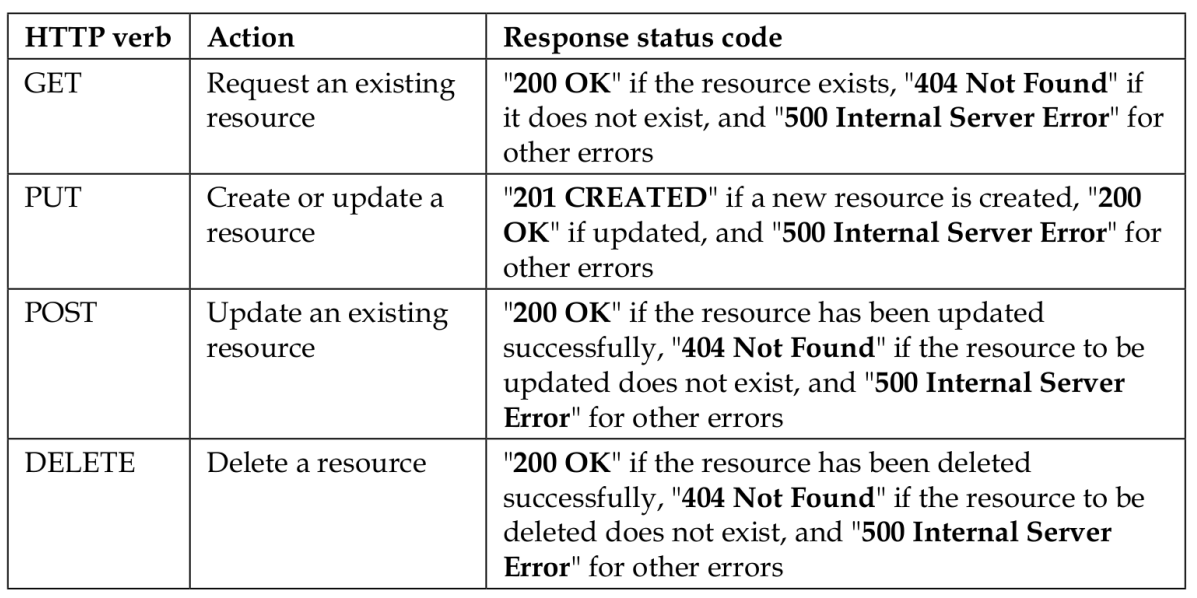
\includegraphics[scale=0.4]{../imagenes/rest.png}
\end{figure}

\newpage
Generalmente nos encontramos como el método POST usado para la creación de recursos, pero en el caso que se crea con una específica URI debe usarse el método PUT:
\begin{verbatim}
PUT /data/documents/balance/22082014 HTTP/1.1
Content-Type: text/xml
Host: www.mydatastore.com
<?xml version="1.0" encoding="utf-8"?>
<balance date="22082014">
<Item>Sample item</Item>
<price currency="EUR">100</price>
</balance>
HTTP/1.1 201 Created
Content-Type: text/xml
Location: /data/documents/balance/22082014
\end{verbatim}
En el caso que sea la aplicación la que decide donde colocar dicho recurso, se usa el método POST:
\begin{verbatim}
POST /data/documents/balance HTTP/1.1
Content-Type: text/xml
Host: www.mydatastore.com
<?xml version="1.0" encoding="utf-8"?>
<balance date="22082014">
<Item>Sample item</Item>
<price currency="EUR">100</price>
</balance>
HTTP/1.1 201 Created
Content-Type: text/xml
Location: /data/documents/balance
\end{verbatim}

\newpage

\subsubsection{Los recursos pueden tener múltiples representaciones}
La representación puede ser variada, por ejemplo usando formato xml o json.
\begin{verbatim}
POST /data/documents/balance HTTP/1.1
Content-Type: application/json
Host: www.mydatastore.com
{
"balance": {
"date": ""22082014"",
"Item": "Sample item",
"price": {
       "-currency": "EUR",
       "#text": "100"
       }
  }
}
HTTP/1.1 201 Created
Content-Type: application/json
Location: /data/documents/balance
\end{verbatim}


\subsubsection{Comunicación sin estado}
\begin{itemize}
\item Todas las operaciones llevadas acabo dentro de una petición HTTP deben ser átomicas.
\item Todas las modificaciones de un recurso deben llevarse a cabo dentro de la misma petición.
\item Después de la petición HTTP, el recurso queda en un estado final.
\item Esto implica que actualizaciones parciales del recurso no se permiten.
\end{itemize}

\newpage

\subsubsection{Confiabilidad}
Los métodos HTTP pueden ser seguros e idempotentes
\begin{description}
\item[Seguros] los métodos HTTP son seguros si las peticiones HTTP no afectan al estado de los recursos, es decir no hay modificaciones ni efectos laterales.
\item[Idempotentes] Cuando la respuesta es siempre la misma, independientemente de las veces que lo llevemos acabo.
\end{description}
\begin{figure}[H]
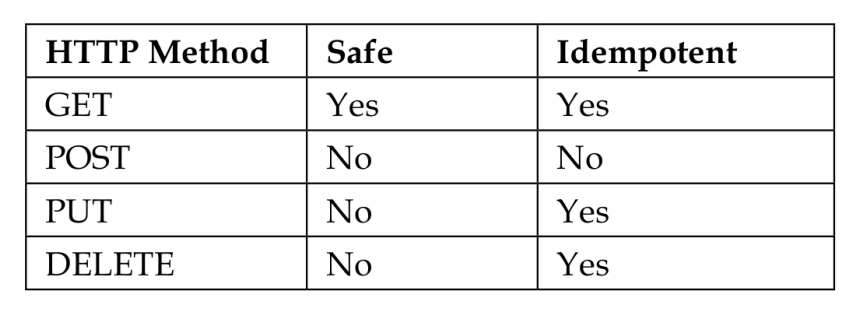
\includegraphics[scale=0.5]{../imagenes/rest1.png}
\end{figure}

\section{Ejemplos de aplicaciones REST}
Ejemplo 1:
\begin{verbatim}
Some sample RESTful API endpoint URLs are as follows:
•	 GET http://myapi.com/v1/accounts : This returns a list of accounts
•	 GET http://myapi.com/v1/accounts/1 : This returns a single account
by Id: 1
•	 POST http://myapi.com/v1/accounts : This creates a new account
(data submitted as a part of the request)
•	 PUT http://myapi.com/v1/accounts/1 : This updates an existing
account by Id: 1 (data submitted as part of the request)
•	 GET http://myapi.com/v1/accounts/1/orders : This returns a list of
orders for account Id: 1
•	 GET http://myapi.com/v1/accounts/1/orders/21345 : This returns the
details for a single order by Order Id: 21345 for account Id: 1
\end{verbatim}
\newpage
Ejemplo 2:
\begin{verbatim}
GET /api/attractions
Retrieves attractions. Takes lat , lng , and radius as querystring parameters and
returns a list of attractions.
GET /api/attraction/:id
Returns an attraction by ID.
POST /api/attraction
Takes lat , lng , name , description , and email in the request body. The newly added
attraction goes into an approval queue.
PUT /api/attraction/:id
Updates an existing attraction. Takes an attraction ID, lat , lng , name , descrip
tion , and email . Update goes into approval queue.
DEL /api/attraction/:id
Deletes an attraction. Takes an attraction ID, email , and reason . Delete goes into
approval queue.
\end{verbatim}
Ejemplo 3:
\begin{figure}[H]
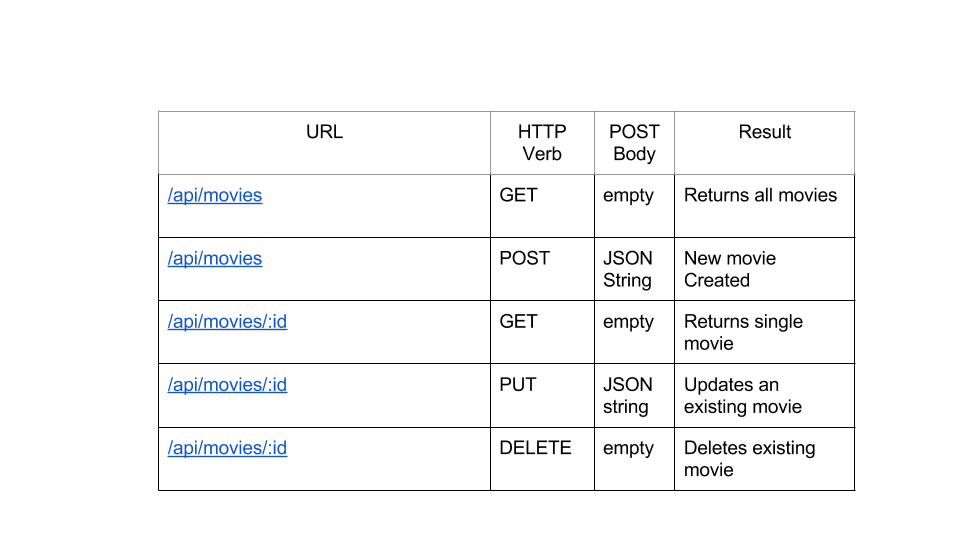
\includegraphics[scale=0.45]{../imagenes/api_rest1.png}
\end{figure}
\newpage
Ejemplo 4:
\begin{figure}[H]
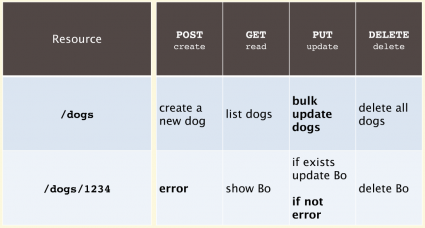
\includegraphics[scale=0.9]{../imagenes/api_rest2.png}
\end{figure}
Ejemplo 5:
\begin{figure}[H]
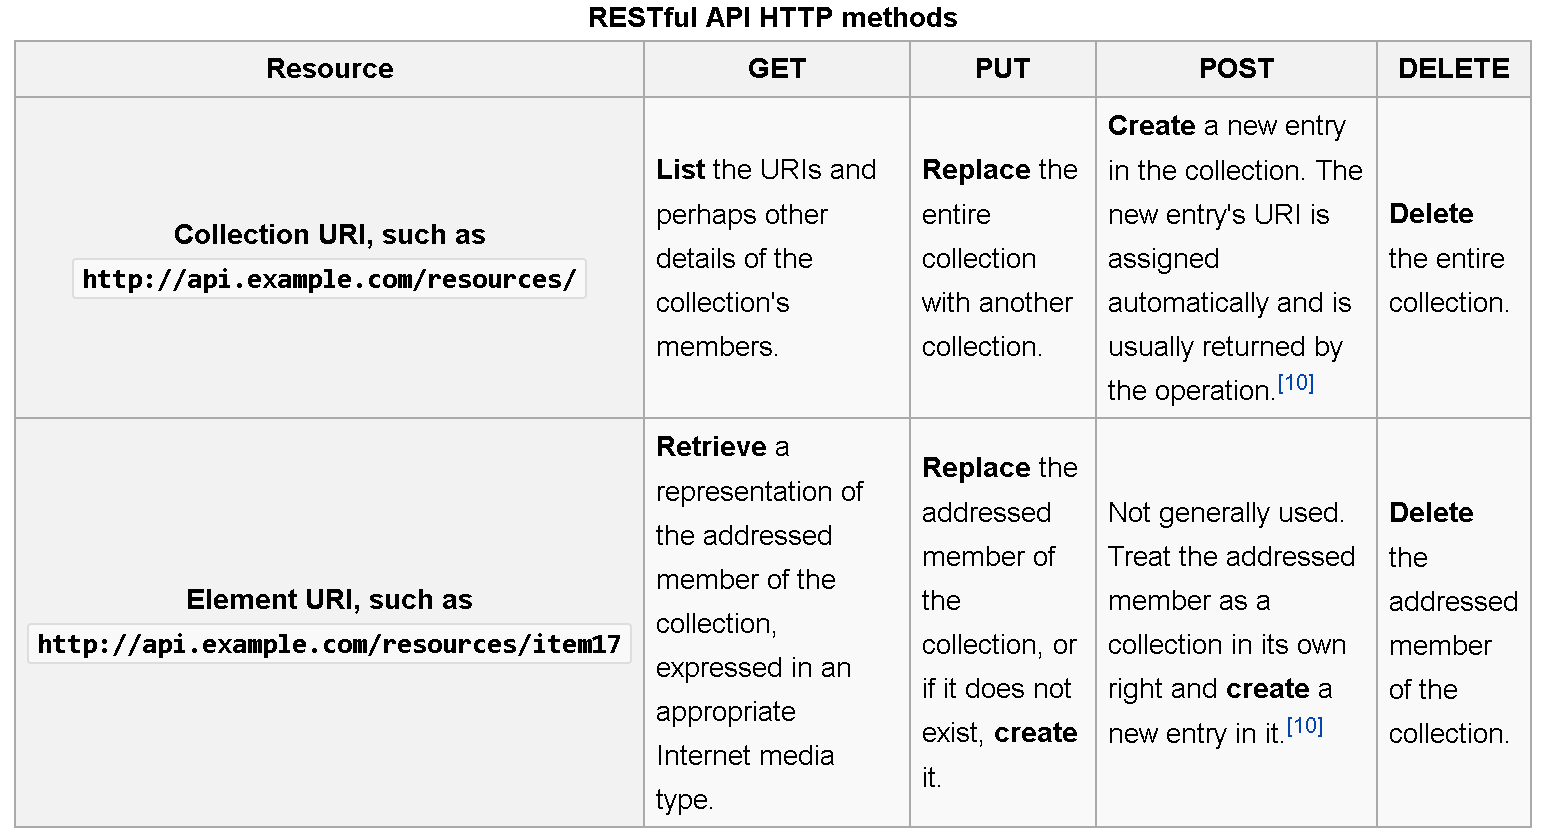
\includegraphics[scale=0.4]{../imagenes/api_rest3.png}
\end{figure}
\newpage
Ejemplo 6:
\begin{figure}[H]
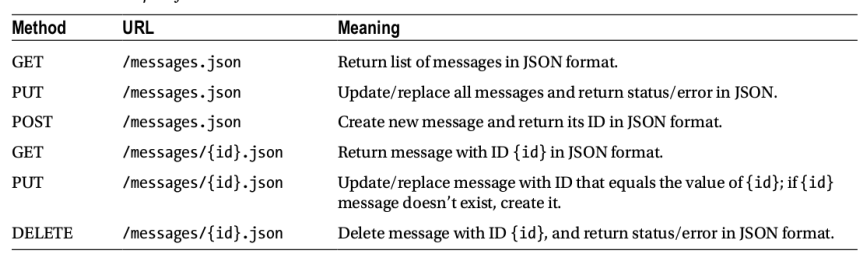
\includegraphics[scale=0.7]{../imagenes/api_rest4.png}
\end{figure}
Ejemplo 7:
\begin{figure}[H]
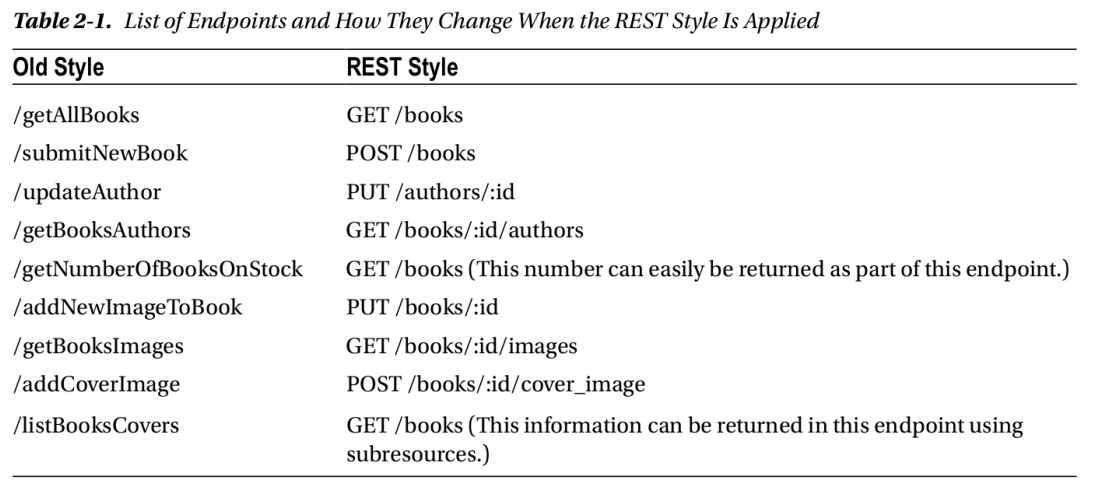
\includegraphics[scale=0.5]{../imagenes/api_rest5.png}
\end{figure}
\newpage
\section{Ejercicio}
Crea la estructura de una aplicación rest para la gestión de usuarios. Los usuarios se identifican por un \emph{id} único y tienen como propiedades nombre, password y profesión.
\\La aplicación debe permitir las siguientes acciones:
\begin{itemize}
\item Listar todos los usuarios.
\item Listar un usuario determinado por loa \emph{id}
\item Borrar un usuario.
\item Añadir un usuario.
\item Actualizar un usuario.
\end{itemize}
Rellena una tabla con el siguiente encabezado:\\
\begin{center}
\begin{tabular}{|c|c|c|c|}
\hline
{\Large URL} & {\Large método HTTP} & {\Large POST body} & {\Large Resultado}\\
\hline
\end{tabular}
\end{center}
\end{document}
